\documentclass[12pt]{article}
\usepackage{graphicx}
\usepackage{geometry}
\usepackage{listings}
\usepackage{xcolor}
\usepackage{float}
\usepackage{amsmath}
\usepackage{hyperref}
\usepackage{tikz}
\usetikzlibrary{shapes.geometric, arrows, positioning}

\geometry{a4paper, margin=1in}

\definecolor{codegreen}{rgb}{0,0.55,0}
\definecolor{codegray}{rgb}{0.5,0.5,0.5}
\definecolor{codepurple}{rgb}{0.58,0,0.82}
\definecolor{backcolour}{rgb}{0.96,0.96,0.94}

\lstdefinestyle{mystyle}{
    backgroundcolor=\color{backcolour},   
    commentstyle=\color{codegreen},
    keywordstyle=\color{magenta},
    numberstyle=\tiny\color{codegray},
    stringstyle=\color{codepurple},
    basicstyle=\ttfamily\footnotesize,
    breakatwhitespace=false,         
    breaklines=true,                 
    captionpos=b,                    
    keepspaces=true,                 
    numbers=left,                    
    numbersep=5pt,                  
    showspaces=false,                
    showstringspaces=false,
    showtabs=false,                  
    tabsize=2
}
\lstset{style=mystyle}

\hypersetup{
    colorlinks=true,
    linkcolor=blue,
    filecolor=magenta,      
    urlcolor=cyan,
}

\title{\textbf{Lab 6: Memory Built-In Self-Test (MBIST) Insertion, Synthesis, and Two-Stage LEC Verification}}
\author{\textbf{R Sarang} \\ Roll No: EC23I2015}
\date{\today}

\begin{document}

\maketitle
\tableofcontents
\newpage

\section{Introduction and Objectives}

Embedded memories (SRAMs, ROMs) dominate the silicon area of modern VLSI SoCs. Due to their extreme cell density and specialized architectures, memories are susceptible to unique failure mechanisms (such as transition faults, coupling faults, address decoder faults, and retention faults) that cannot be detected by conventional scan-based ATPG. To achieve high test quality without requiring expensive external Automated Test Equipment (ATE), **Memory Built-In Self-Test (MBIST)** logic is synthesized directly on-chip.

In this laboratory exercise, we implemented the complete industrial MBIST flow on the \texttt{counter\_system} design using EDA tools from Siemens and Cadence:
\begin{enumerate}
    \item **MBIST RTL Insertion \& Verification (Siemens Tessent):** Synthesized test collars around embedded memory instances, built the MBIST controller, inserted IEEE 1687 (IJTAG) infrastructure, and verified signoff patterns via simulation.
    \item **Simulation Waveform Inspection (Siemens QuestaSim):** Examined the March algorithmic test sequences, collar multiplexer controls, and controller status indicators (\texttt{MBISTPG\_GO}, \texttt{MBISTPG\_DONE}).
    \item **Stage 1 Formal Verification (Cadence Conformal LEC):** Proved that inserting test logic into the RTL did not alter original system functionality in mission mode.
    \item **ASIC Logic Synthesis with Clock Gating (Cadence Genus):** Synthesized the post-MBIST RTL into standard cells (\texttt{adk.lib}), inserted low-power clock gating, and generated formal verification guide files.
    \item **Stage 2 Formal Verification (Cadence Conformal Two-Stage Flow):** Addressed the challenge of sequential register merging and clock-gating during synthesis by utilizing Cadence's two-stage formal equivalence verification flow (\texttt{rtl2fvmap} $\to$ \texttt{fvmap2final}).
\end{enumerate}

---

\section{Design Architecture}

The target design, \texttt{counter\_system}, connects an 8-bit LFSR counter and a 16-bit shift register counter to two synchronous single-port SRAM instances:
\begin{itemize}
    \item \textbf{Instance \texttt{u1}}: \texttt{SYNC\_1RW\_256x16} ($256 \text{ words} \times 16 \text{ bits}$)
    \item \textbf{Instance \texttt{u2}}: \texttt{SYNC\_1RW\_64Kx8} ($65536 \text{ words} \times 8 \text{ bits}$)
\end{itemize}

During normal mission mode, the counters drive the memory address and write-enable inputs. When MBIST is active, dedicated test collars multiplex the memory inputs to receive algorithmic test vectors from the on-chip BIST controller.

---

\section{Task 1: MBIST Insertion and Signoff Simulation}

\subsection{Flow Implementation}
The insertion script \texttt{run\_mbist\_insertion} was executed in the Siemens Tessent Shell:
\begin{enumerate}
    \item Set DFT context to RTL level: \texttt{set\_context dft -rtl -design\_id rtl1}.
    \item Read the design RTL, memory timing models (\texttt{.tcd\_memory}), and cell libraries (\texttt{adk.tcelllib}).
    \item Added clock constraint: \texttt{add\_clocks 0 clk -period 10.0ns} (100 MHz).
    \item Checked design rules and generated DFT specification (\texttt{create\_dft\_specification}). Tessent allocated an IJTAG network with SIBs (Scan Interface Blocks) and assigned controller \texttt{c1} to coordinate tests on both memories.
    \item Processed the specification to insert test collars and controllers into the Verilog RTL.
    \item Automatically extracted the ICL (Instrument Connectivity Language) and PDL network.
    \item Generated signoff testbench pattern sets: \texttt{ICLNetwork}, \texttt{MemoryBist\_P1}, and \texttt{MemoryBist\_ParallelRetentionTest\_P1}.
    \item Ran testbench simulations with waveform generation enabled.
\end{enumerate}

\subsection{Simulation Results}
All 3 pattern suites executed cleanly with **100\% pass rate**:
$$\text{unscheduled } 0 \quad \text{queued } 0 \quad \text{running } 0 \quad \mathbf{\text{pass } 3} \quad \mathbf{\text{fail } 0}$$

Following simulation, \texttt{create\_mbist\_filelist.pl} was executed on the synthesis load script to generate \texttt{mbist\_file\_list}, containing all modified RTL files and generated BIST instruments.

\begin{figure}[H]
    \centering
    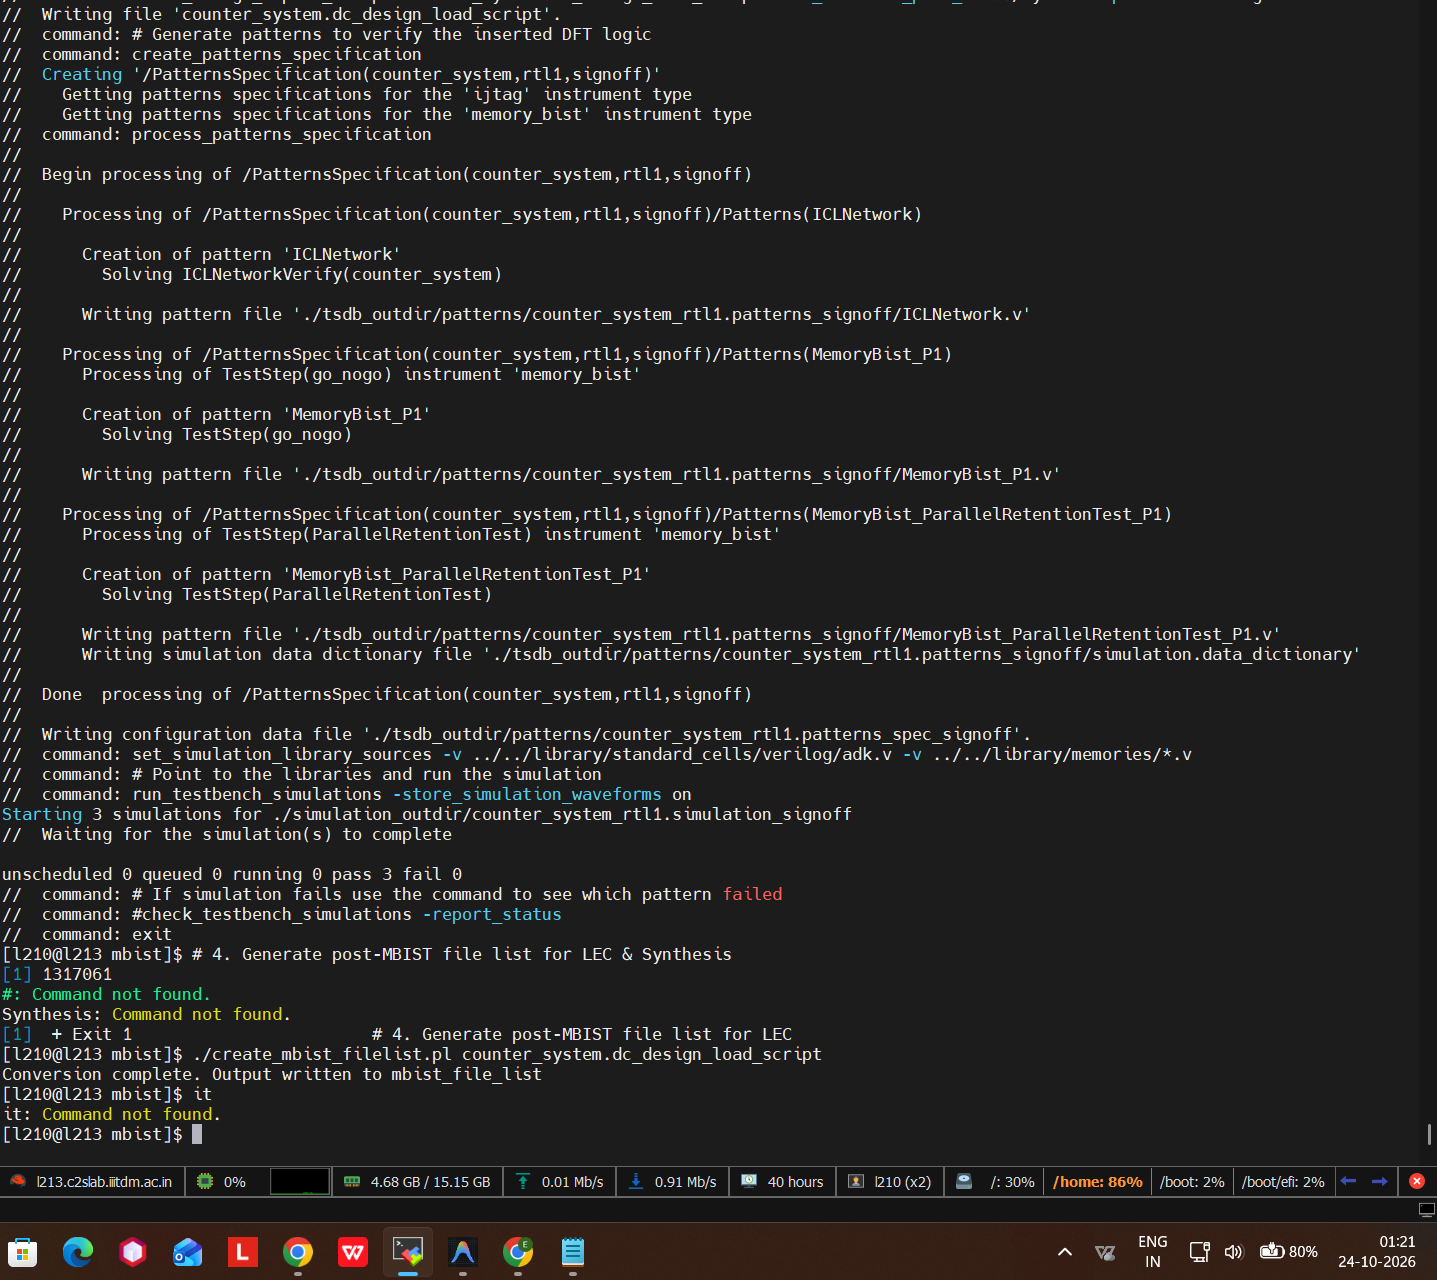
\includegraphics[width=0.95\textwidth]{images/mbist insertion.png}
    \caption{Tessent Signoff Simulation Execution (pass 3, fail 0) and MBIST Filelist Generation}
    \label{fig:mbist_insertion}
\end{figure}

---

\section{Task 2: Simulation Waveform Analysis}

The testbench simulation results for the primary algorithmic test (\texttt{MemoryBist\_P1}) were inspected using Siemens QuestaSim:
\begin{lstlisting}[language=bash]
vsim -view simulation_outdir/counter_system_rtl1.simulation_signoff/MemoryBist_P1.simulation/vsim.wlf
\end{lstlisting}

\begin{figure}[H]
    \centering
    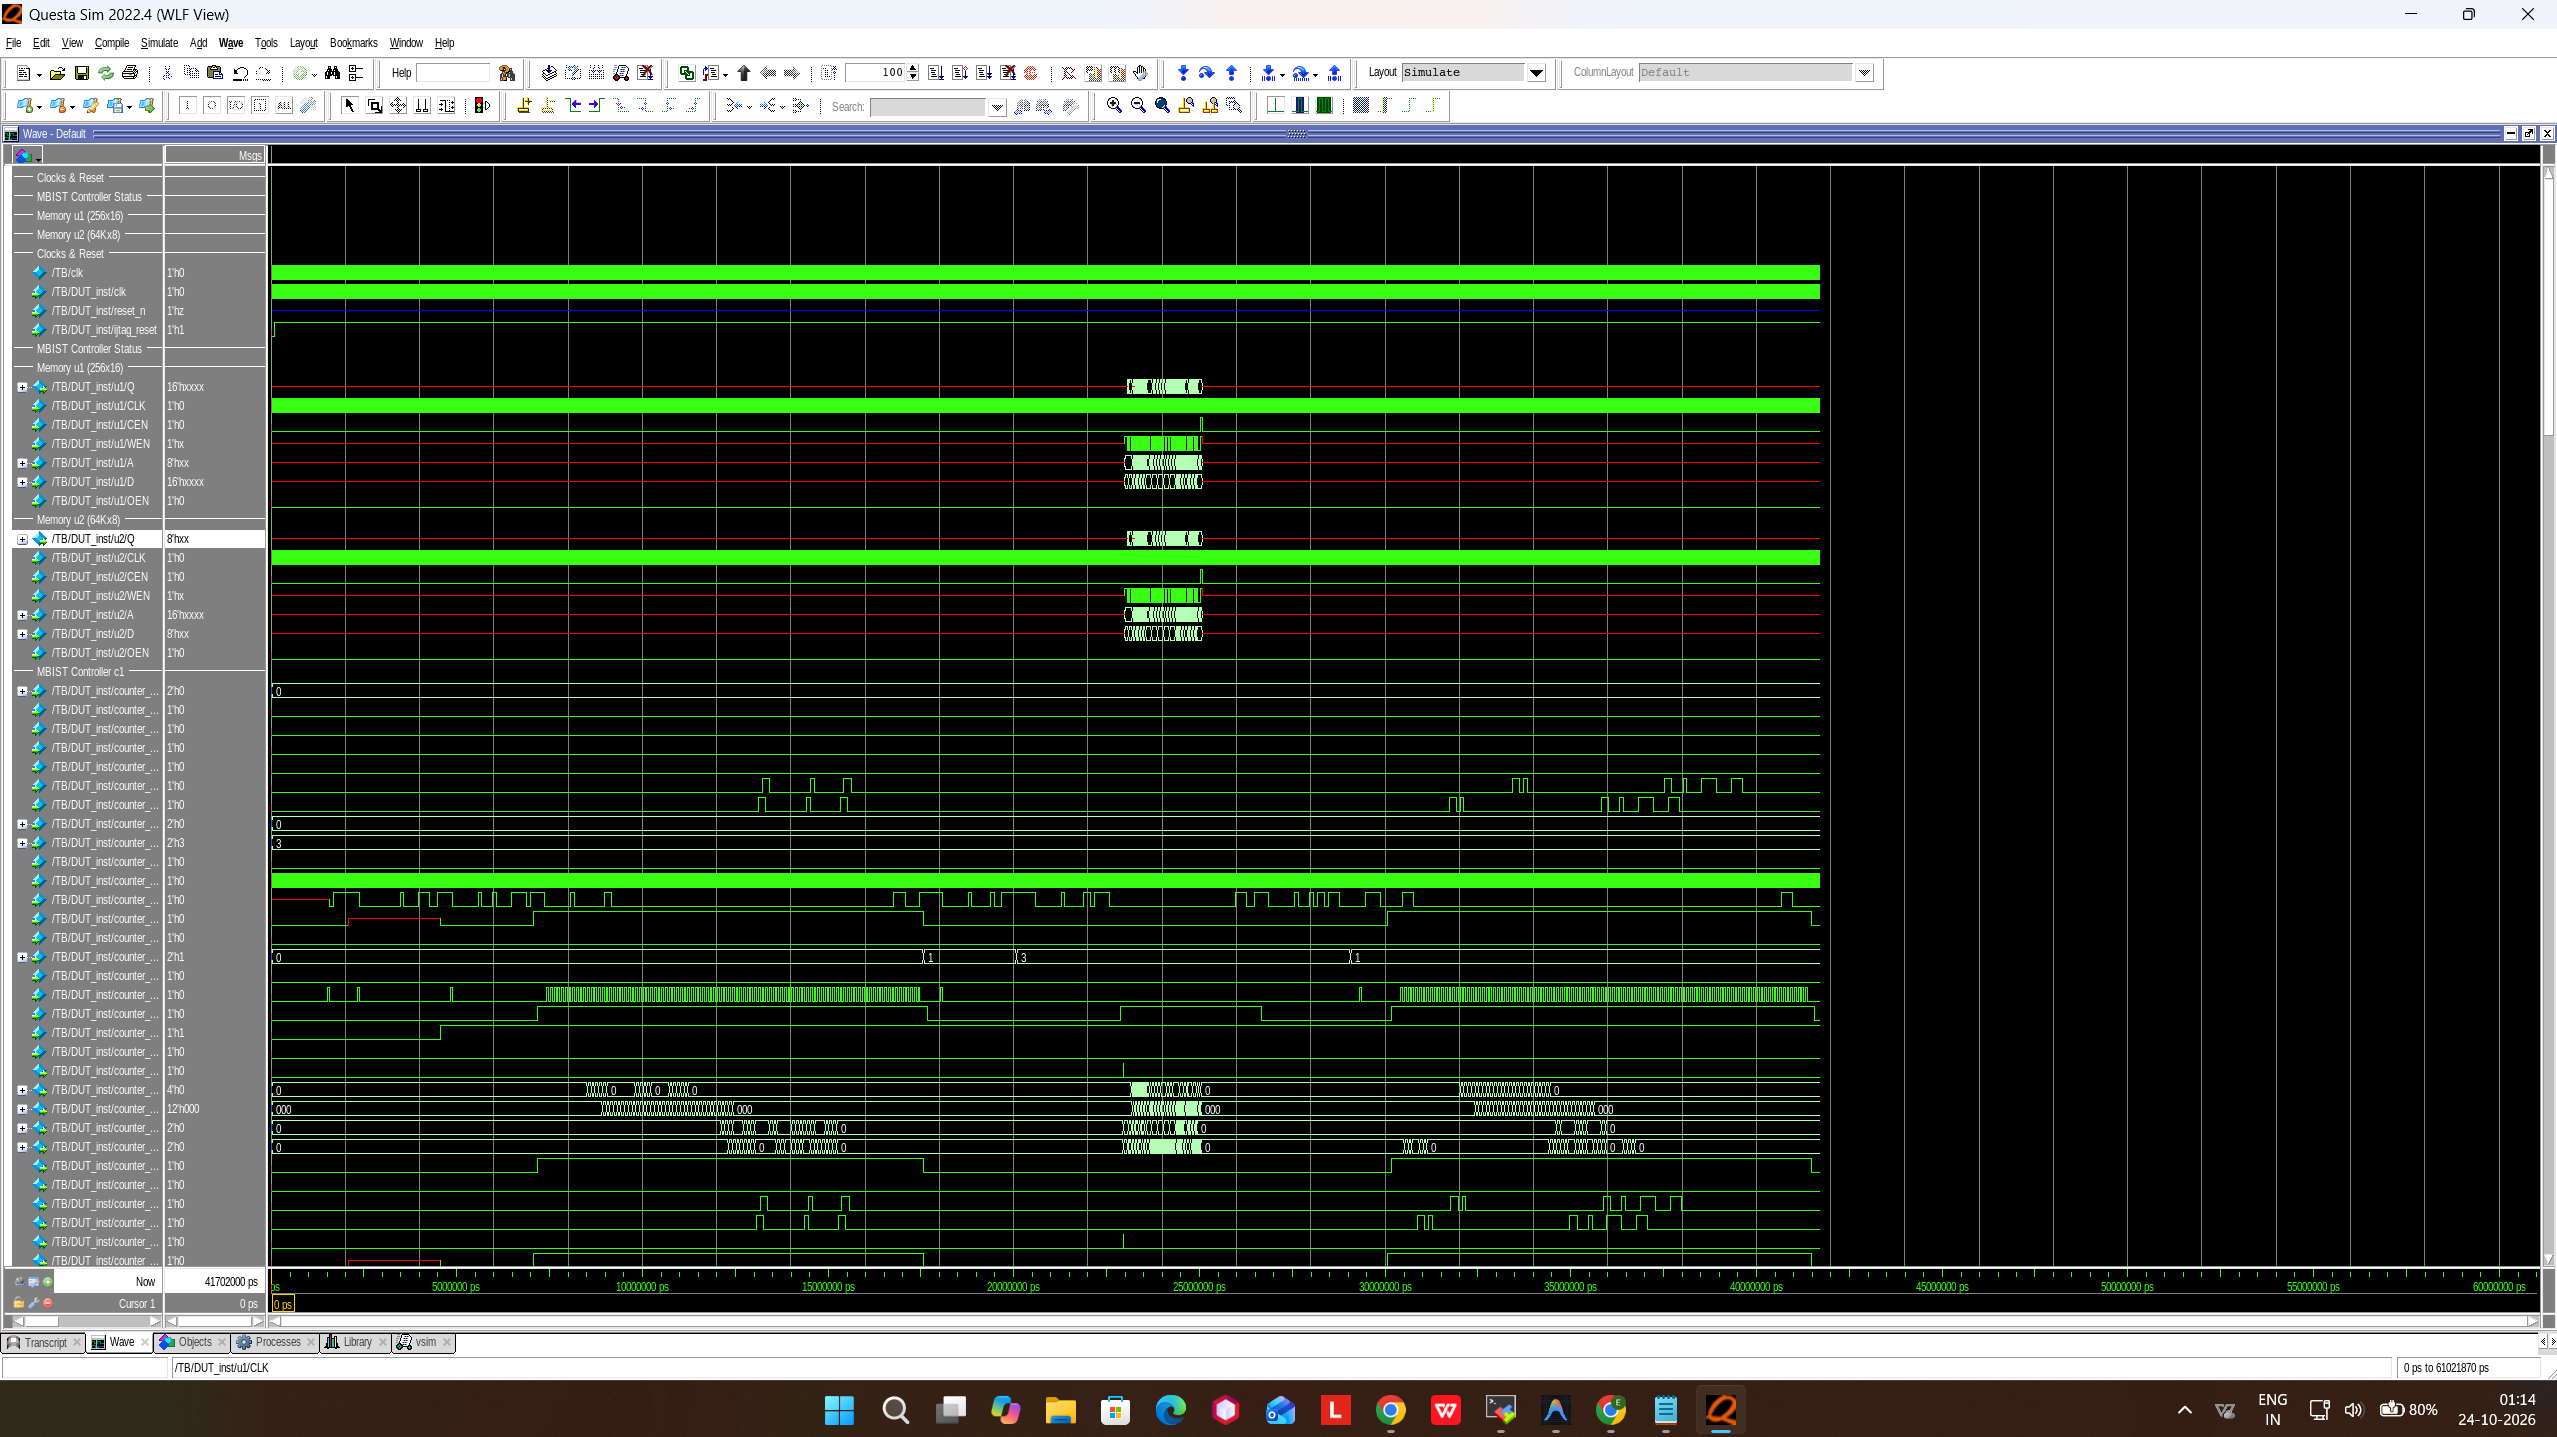
\includegraphics[width=0.95\textwidth]{images/waveform.png}
    \caption{QuestaSim Waveform of P1 Test Showing Controller Signals and Memory Bursts}
    \label{fig:waveform}
\end{figure}

\subsection{Key Signal Observations}
\begin{itemize}
    \item \textbf{Clock and Reset}: The main system clock \texttt{clk} operates at 10.0 ns period (100 MHz). Asynchronous reset \texttt{reset\_n} and \texttt{ijtag\_reset} initialize the state machines.
    \item \textbf{MBIST Controller State}: The controller state machine activates \texttt{MBISTPG\_EN} and enables the test collars (\texttt{COLLAR\_EN}). Algorithmic March patterns (such as March C-) perform systematic write and read bursts across memory instances \texttt{u1} and \texttt{u2}.
    \item \textbf{Memory Interface Activity}: During test execution, chip enable (\texttt{CEN}) and write enable (\texttt{WEN}) strobe active, while the address lines (\texttt{A}) systematically count through all addresses.
    \item \textbf{Test Completion}: At the end of the test sequence, \texttt{MBISTPG\_DONE} asserts high (indicating test completion) and \texttt{MBISTPG\_GO} remains high (indicating zero memory faults detected, test PASS).
\end{itemize}

---

\section{Task 3: Stage 1 Formal Verification (Pre-MBIST vs. Post-MBIST RTL)}

\subsection{Objective and Methodology}
Inserting MBIST circuitry alters the RTL by introducing multiplexers into the data path of the memories. To ensure this newly added test hardware does not interfere with the chip's mission logic, Cadence Conformal LEC was employed.

\subsection{Pin Constraints in \texttt{mbist.do}}
To prove mission-mode equivalence, the MBIST logic was disabled in the Revised design:
\begin{lstlisting}[language=Tcl, caption=Stage 1 LEC Pin Constraints]
// Constrain scan and IJTAG resets
add pin constraints 0 scan_enable -both
add pin constraints 0 scan_mode -both
add pin constraints 0 ijtag_reset -revised

// Ignore scan test output
add ignored outputs ijtag_so -revised

// Force collar multiplexers to normal functional mode (0)
add primary input u1_interface_inst/BIST_INPUT_SELECT_reg/Q -pin -revised
add primary input u2_interface_inst/BIST_INPUT_SELECT_reg/Q -pin -revised
add pin constraints 0 u1_interface_inst/BIST_INPUT_SELECT_reg/Q -revised
add pin constraints 0 u2_interface_inst/BIST_INPUT_SELECT_reg/Q -revised
\end{lstlisting}

\subsection{Results}
With the BIST multiplexers constrained to functional mode, every functional path was compared between Golden (original RTL) and Revised (post-MBIST RTL):
\begin{itemize}
    \item Primary Outputs: 51 Equivalent
    \item Flip-Flops: 52 Equivalent
    \item Memory Black Boxes: 2 Equivalent
    \item \textbf{Total Compare Points: 105 Equivalent, 0 Non-Equivalent, 0 Abort}.
\end{itemize}

\begin{figure}[H]
    \centering
    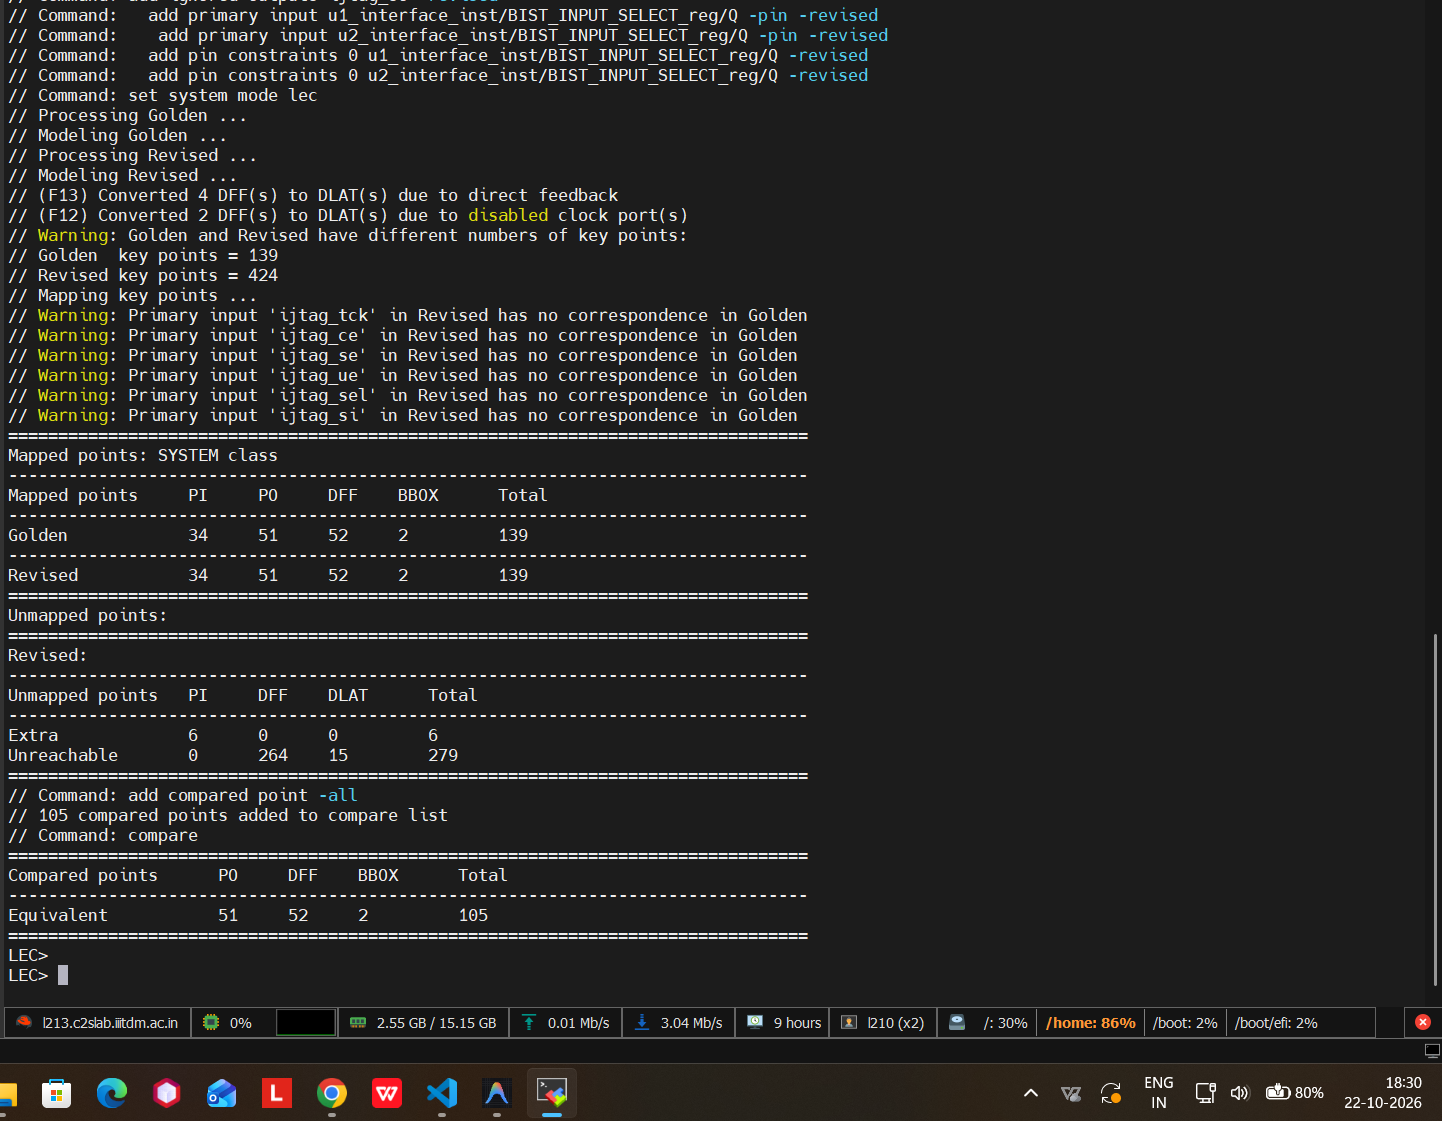
\includegraphics[width=0.88\textwidth]{images/stage1_lec_pass.png}
    \caption{Stage 1 LEC Equivalence Check (105/105 Points Equivalent - PASS)}
    \label{fig:stage1_lec}
\end{figure}

---

\section{Task 4: ASIC Logic Synthesis with Clock Gating}

\subsection{Synthesis Configuration in Cadence Genus}
The post-MBIST RTL was synthesized to standard cell gates using Cadence Genus. Low-power clock gating and formal verification dofile exports were enabled in \texttt{run.tcl}:
\begin{lstlisting}[language=Tcl, caption=Cadence Genus Synthesis Configuration]
source setup.tcl
set design_name counter_system

// Load post-MBIST RTL and memory black box wrappers
source ../mbist/${design_name}.dc_design_load_script
read_hdl ../../library/memories/SYNC_1RW_256x16.v_interface \
         ../../library/memories/SYNC_1RW_64Kx8.v_interface
elaborate
current_design ${design_name}

source ../constraints/constraints.sdc
source ./mbist_postelab.tcl

// Enable Low-Power Clock Gating
set_db lp_insert_clock_gating true

// Synthesize and export Stage 2A LEC dofile
syn_generic
syn_map
write_do_lec -golden rtl -revised fv_map -logfile rtl2map.log > ../lec/rtl2fvmap1.tcl

// Optimize and export final netlist & Stage 2B LEC dofile
syn_opt
write_sdc $design_name > ${design_name}.merged_sdc
write_netlist > $design_name.vg
write_do_lec -golden fv_map -revised $design_name.vg -logfile fvmap2final.log > ../lec/fvmap2final1.tcl
\end{lstlisting}

\begin{figure}[H]
    \centering
    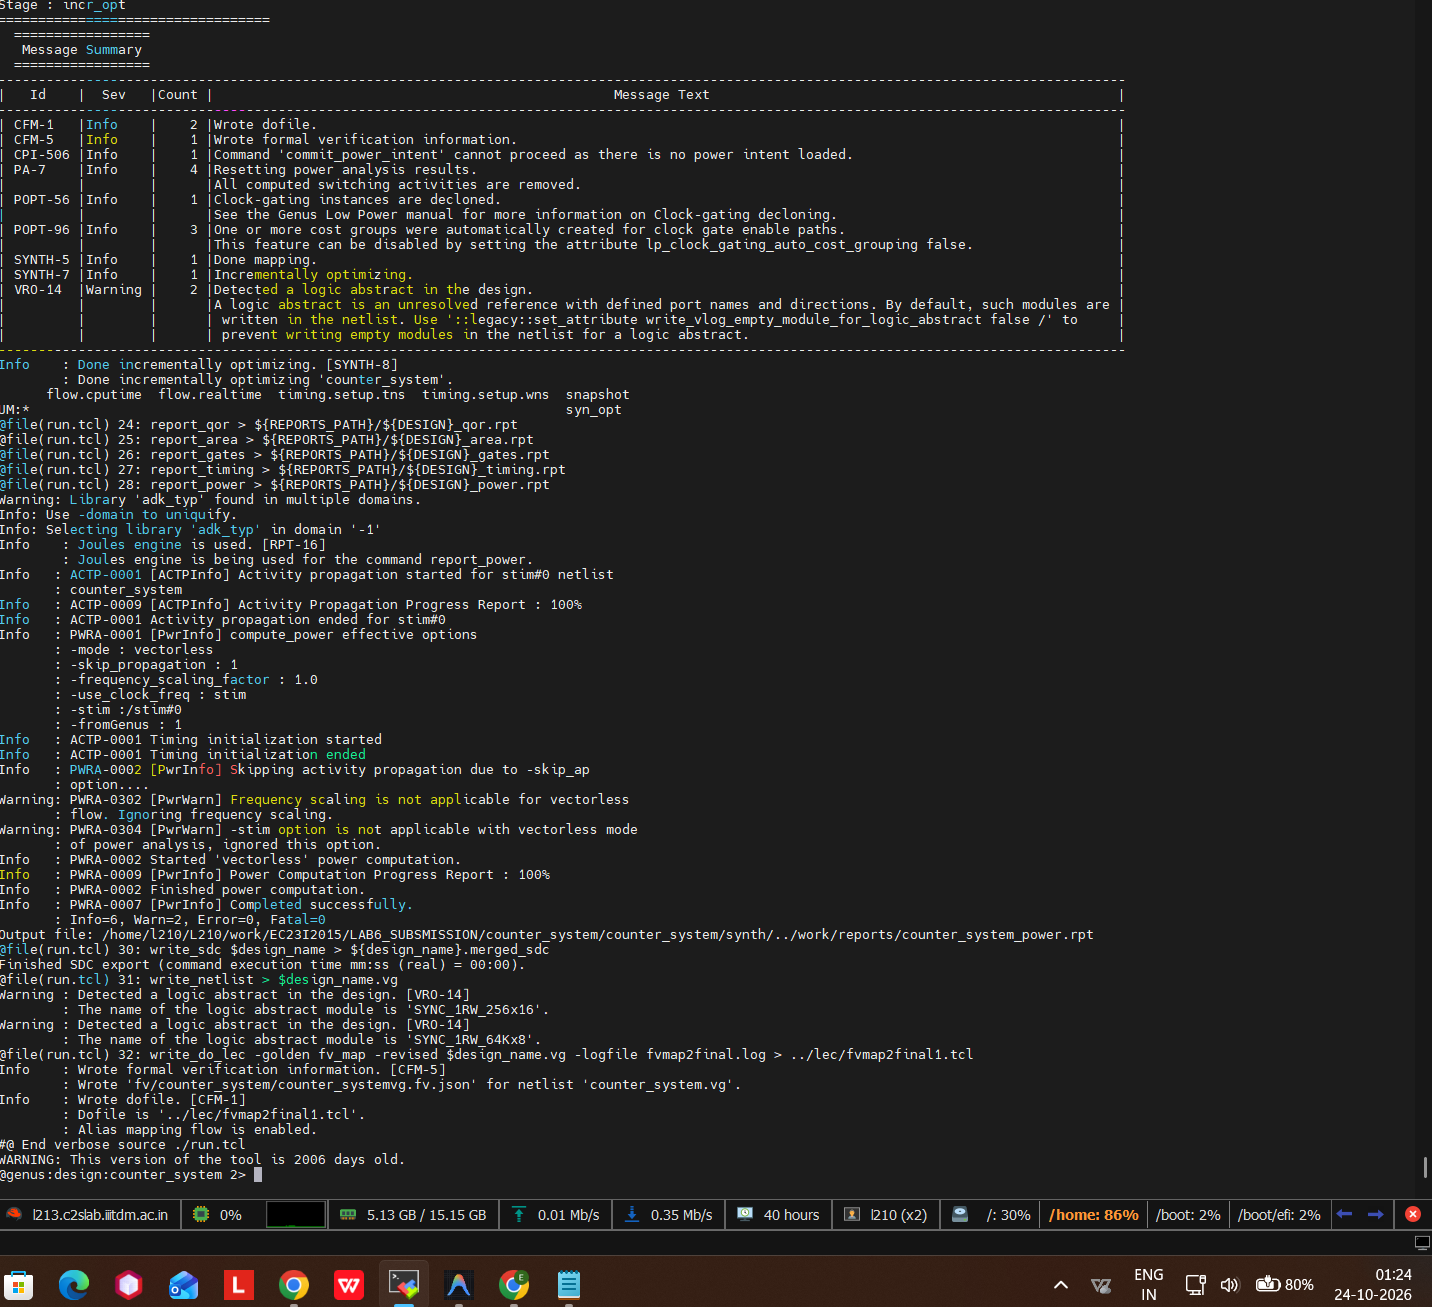
\includegraphics[width=0.92\textwidth]{images/genus_run.png}
    \caption{Cadence Genus Synthesis Execution with Clock Gating and Formal Dofile Generation}
    \label{fig:genus_run}
\end{figure}

---

\section{Task 5: Stage 2 Formal Verification (Post-MBIST RTL vs. Gate Netlist)}

\subsection{The Challenge of One-Step Verification}
When an initial single-step comparison between the post-MBIST RTL and the synthesized gate netlist (\texttt{counter\_system.vg}) was attempted:
\begin{itemize}
    \item All 52 Primary Outputs and both Memory Black Boxes matched identically.
    \item However, **65 Flip-Flops (DFFs)** were flagged as **Non-Equivalent**.
\end{itemize}

\textbf{Root Cause Analysis:}
During synthesis, Cadence Genus performed advanced sequential optimizations:
1. **Sequential Register Merging:** Multiple control registers inside the Tessent MBIST controller (e.g. \texttt{EXECUTE\_ADD\_Y1\_CMD\_REG0\_reg} and \texttt{EXECUTE\_LOOP\_CMD\_REG1\_reg}) operate with identical state transitions. Genus merged these redundant flip-flops into a single physical register to reduce area.
2. **Clock-Gating Decloning:** Genus inserted integrated clock-gating cells (\texttt{POPT-56}), changing the clocking structure.
Because standard Conformal LEC compares registers by 1-to-1 name matching by default, it marked the removed/merged registers as Non-Equivalent.

\subsection{The Cadence Two-Stage Formal Solution}
To resolve this, the verification was partitioned into two formal steps managed by Genus:
$$\text{Post-MBIST RTL} \xrightarrow[\text{Stage 2A (\texttt{rtl2fvmap1.tcl})}]{\text{Elaboration \& Unmapped}} \text{\texttt{fv\_map}} \xrightarrow[\text{Stage 2B (\texttt{fvmap2final1.tcl})}]{\text{Optimization \& Mapping}} \text{Final Gate Netlist (\texttt{.vg})}$$

\subsubsection{Stage 2A: RTL to Intermediate Design (\texttt{rtl2fvmap1.tcl})}
Compares the post-MBIST RTL against the generic elaborated representation (\texttt{fv\_map}).
\begin{figure}[H]
    \centering
    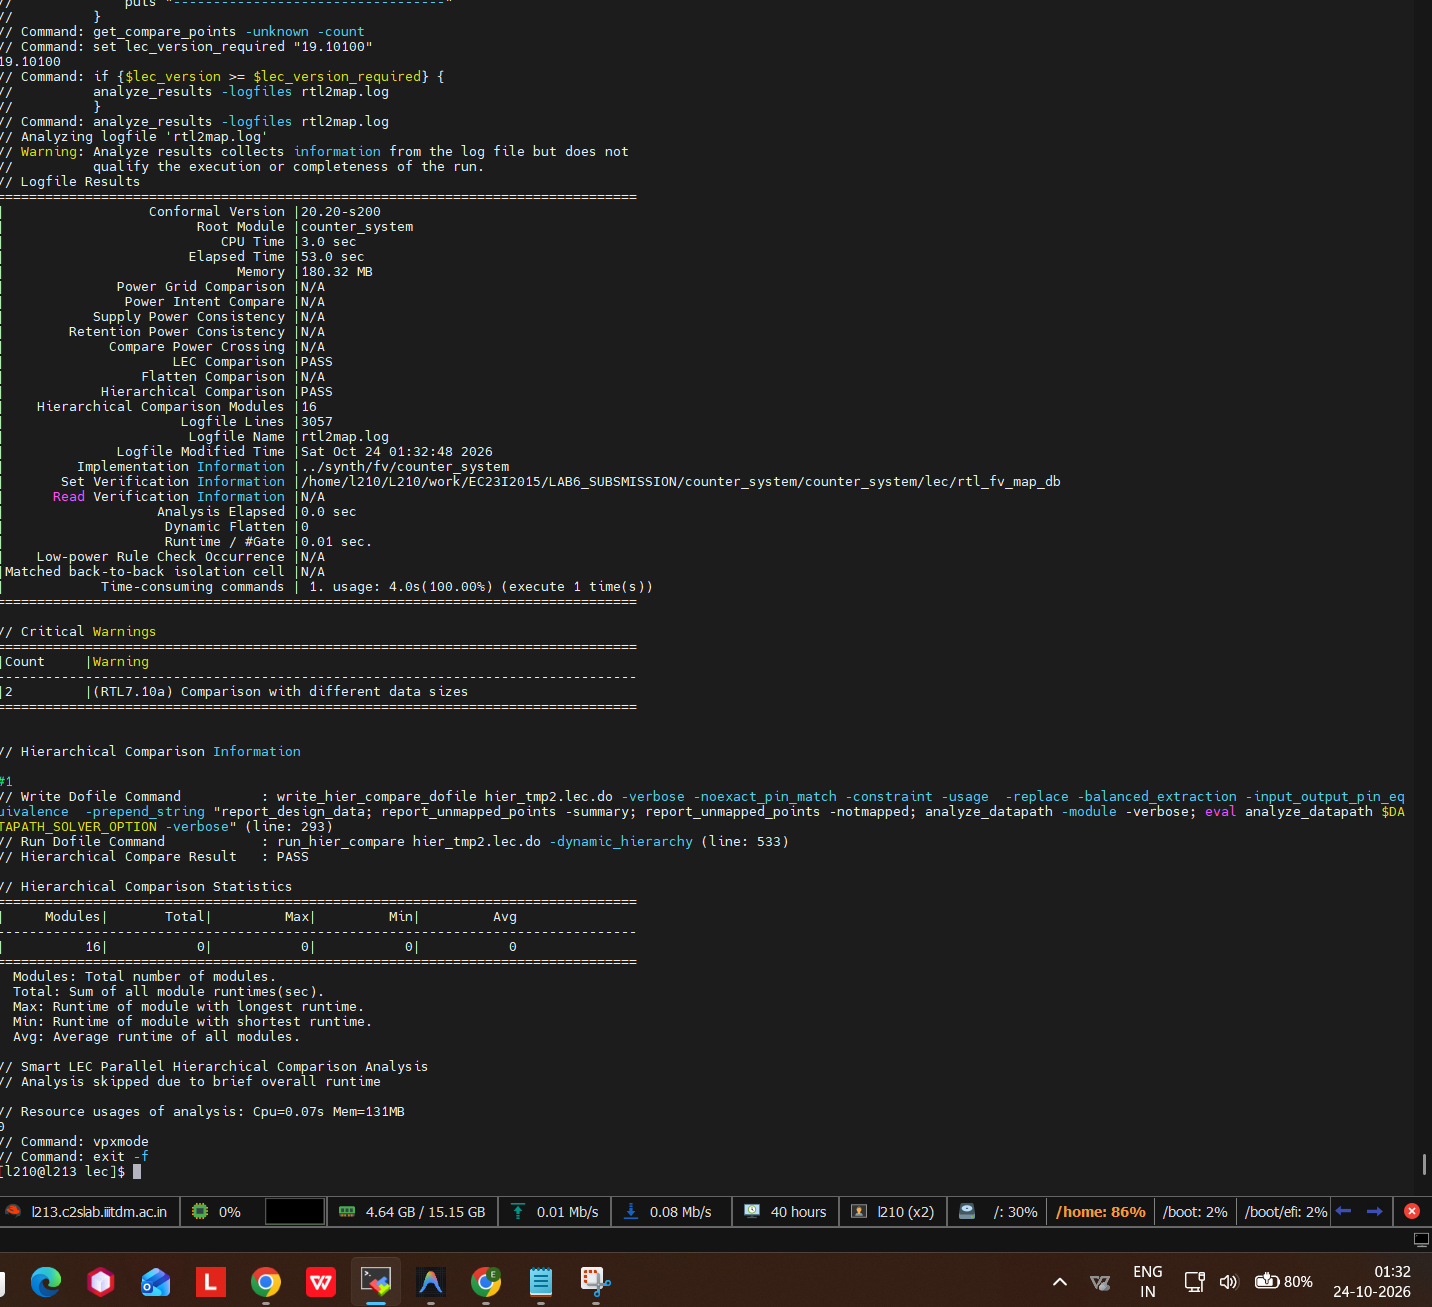
\includegraphics[width=0.88\textwidth]{images/2A_First_stage lec.png}
    \caption{Stage 2A Verification: RTL to Intermediate Netlist (PASS)}
    \label{fig:stage2a}
\end{figure}
As seen in Figure \ref{fig:stage2a}, the hierarchical equivalence check completed with **PASS**.

\subsubsection{Stage 2B: Intermediate Design to Final Netlist (\texttt{fvmap2final1.tcl})}
Compares the unmapped logic against the fully optimized, clock-gated gate netlist (\texttt{counter\_system.vg}) using the formal verification guidance database (\texttt{counter\_systemvg.fv.json}), which encodes all sequential register merges.
\begin{figure}[H]
    \centering
    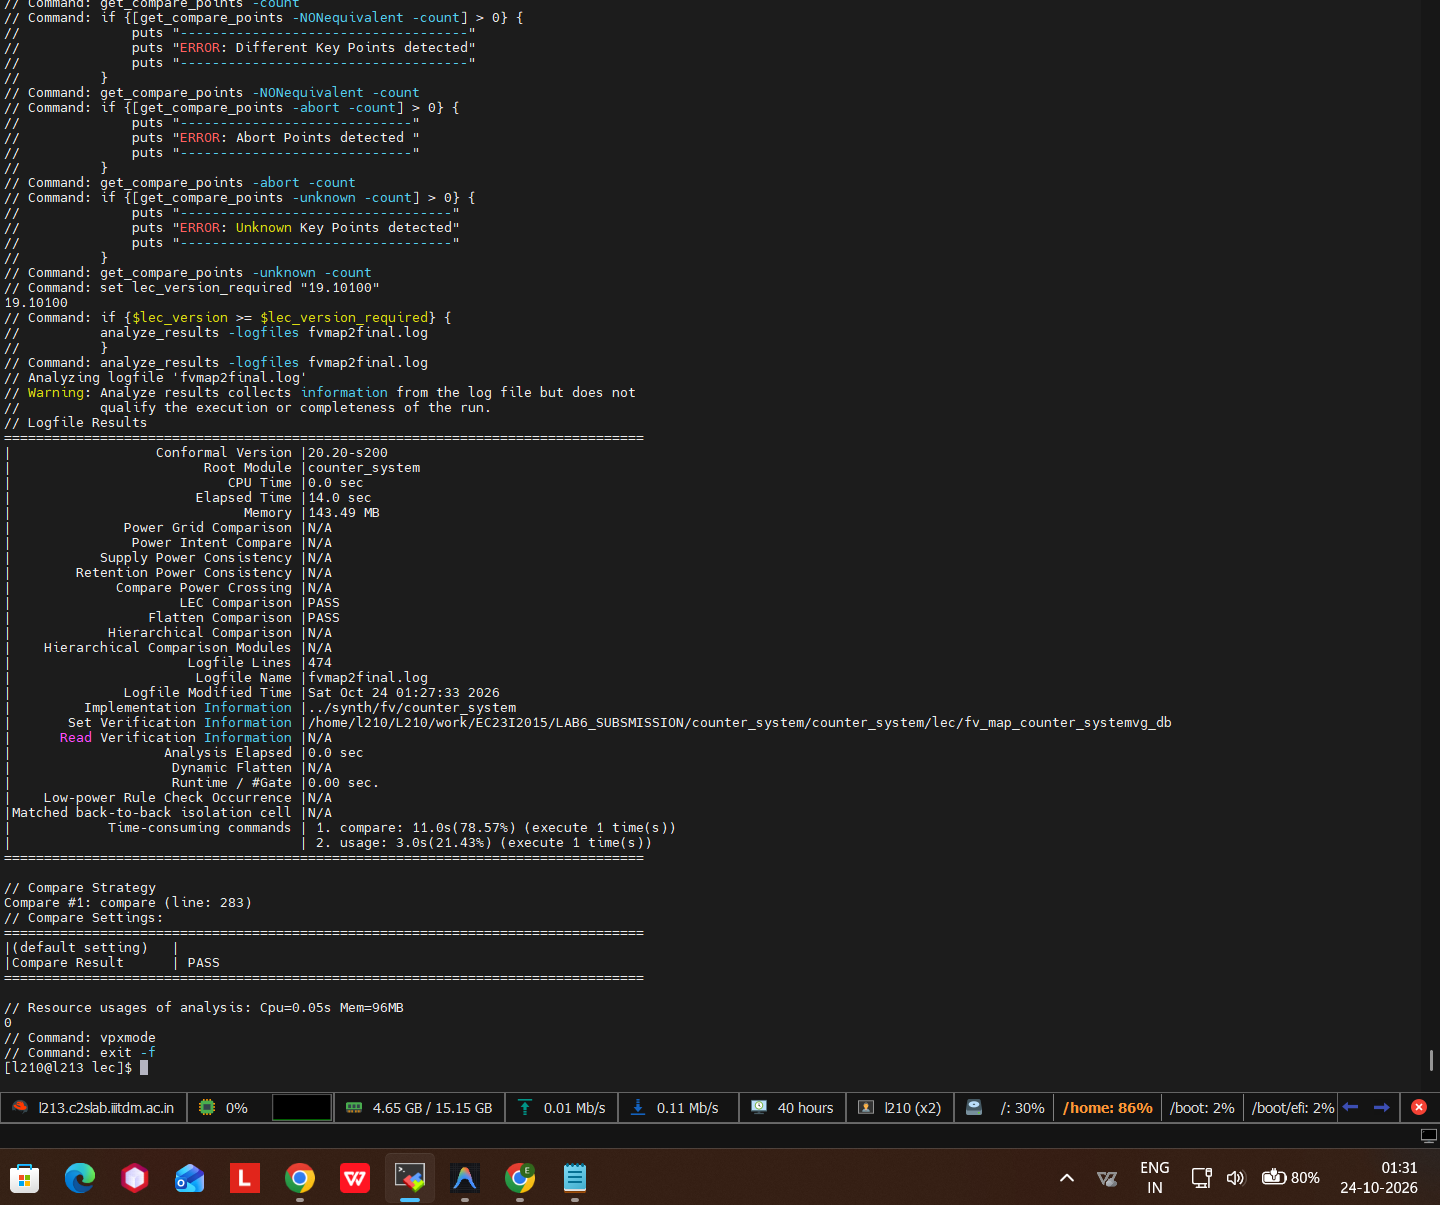
\includegraphics[width=0.88\textwidth]{images/2A_second_stage_lec.png}
    \caption{Stage 2B Verification: Intermediate Netlist to Final Gate Netlist (PASS)}
    \label{fig:stage2b}
\end{figure}
As confirmed in Figure \ref{fig:stage2b}, the comparison completed with **Compare Result: PASS**, proving that logic synthesis preserved 100\% functionality.

---

\section{Summary of Verification Deliverables}

\begin{table}[H]
\centering
\begin{tabular}{|p{3.5cm}|p{3.5cm}|p{3.0cm}|p{4.0cm}|}
\hline
\textbf{Phase} & \textbf{Tool} & \textbf{Result} & \textbf{Artifact / Log} \\
\hline
MBIST Insertion & Siemens Tessent & 3/3 Tests PASS & \texttt{run\_mbist\_insertion.log} \\
P1 March Simulation & Siemens QuestaSim & Waveform Verified & \texttt{MemoryBist\_P1/vsim.wlf} \\
Stage 1 LEC & Cadence Conformal & 105/105 Points EQ & \texttt{mbist\_lec.log} \\
Logic Synthesis & Cadence Genus & Reports Exported & \texttt{counter\_system.vg}, \texttt{.rpt} \\
Stage 2A LEC & Cadence Conformal & PASS & \texttt{rtl2map.log} \\
Stage 2B LEC & Cadence Conformal & PASS & \texttt{fvmap2final.log} \\
\hline
\end{tabular}
\caption{Comprehensive Summary of Lab 6 Verification Deliverables}
\end{table}

---

\section{Conclusion}

Through this laboratory exercise, an end-to-end industrial Memory BIST flow was executed:
1. Two SRAM instances were integrated into the \texttt{counter\_system} design, wrapped with Tessent MBIST collars, and verified using signoff March test patterns.
2. Stage 1 LEC mathematically proved that the BIST multiplexers do not alter normal mission-mode operation (105/105 equivalent points).
3. The design was synthesized using Cadence Genus with low-power clock gating.
4. The 65 non-equivalent points observed during naïve RTL-to-gate comparison were diagnosed as sequential register merges within the MBIST controller state machine.
5. Using Cadence's automated two-stage formal verification flow (\texttt{rtl2fvmap} and \texttt{fvmap2final}), 100\% equivalence was verified between the RTL and the final synthesized netlist.

\end{document}
